\documentclass[a4paper,12pt]{article}
\usepackage{anysize}
\usepackage[T1]{fontenc}
\usepackage[stable]{footmisc}
\usepackage{setspace}
\usepackage{lmodern}
\usepackage{libertine}
\usepackage[libertine]{newtxmath}
\usepackage[scale=0.825]{FiraMono}
\usepackage[top=2cm,bottom=2cm,left=2cm,right=2cm]{geometry}
\usepackage{mathtools}
\usepackage[authoryear]{natbib}
\usepackage[USenglish]{babel}
\usepackage[USenglish]{isodate}
\usepackage{babelbib}
\usepackage{graphicx}
\usepackage{booktabs, makecell, longtable}
\usepackage{dcolumn}
\usepackage{float}
\usepackage[caption = false]{subfig}
\floatplacement{figure}{H}
\usepackage{caption}
\usepackage{rotating}
\usepackage{pdflscape}
\usepackage{pdflscape}
\newcommand{\blandscape}{\begin{landscape}}
\newcommand{\elandscape}{\end{landscape}}
\usepackage{ifthen}
\usepackage{graphicx}
\usepackage{markdown}
\usepackage[usenames,dvipsnames]{xcolor}
\definecolor{darkblue}{rgb}{0.0,0.0,0.55}
\usepackage{tikz}
\usetikzlibrary{shapes.geometric, arrows}
\setcitestyle{aysep={}}
\usepackage{etoolbox}
\makeatletter
\patchcmd{\NAT@citex}
  {\@citea\NAT@hyper@{%
	 \NAT@nmfmt{\NAT@nm}%
	 \hyper@natlinkbreak{\NAT@aysep\NAT@spacechar}{\@citeb\@extra@b@citeb}%
	 \NAT@date}}
  {\@citea\NAT@nmfmt{\NAT@nm}%
   \NAT@aysep\NAT@spacechar\NAT@hyper@{\NAT@date}}{}{}
\patchcmd{\NAT@citex}
  {\@citea\NAT@hyper@{%
	 \NAT@nmfmt{\NAT@nm}%
	 \hyper@natlinkbreak{\NAT@spacechar\NAT@@open\if*#1*\else#1\NAT@spacechar\fi}%
   {\@citeb\@extra@b@citeb}%
	 \NAT@date}}
  {\@citea\NAT@nmfmt{\NAT@nm}%
   \NAT@spacechar\NAT@@open\if*#1*\else#1\NAT@spacechar\fi\NAT@hyper@{\NAT@date}}
  {}{}
\makeatother
\cleanlookdateon
\exhyphenpenalty=1000
\hyphenpenalty=1000
\widowpenalty=1000
\clubpenalty=1000
\usepackage{hyperref}

\hypersetup{
	breaklinks=true,
	linkcolor=darkblue,
	citecolor=darkblue,
	urlcolor=darkblue,
	colorlinks=true}

\doublespacing

\title{{\Large Writing Sample} \\ Legislative Outcomes and Malapportionment: \\ Evidence from Latin America\thanks{I thank Prof. Umberto Mignozzetti and Dr. Danilo Freire for their guidance and helpful comments. Replication materials are available at \url{https://github.com/catarinaroman/malapportionment-lat-am}.}}

\vspace{2cm}

\author{Catarina Roman\thanks{University of São Paulo, \href{mailto:catarinamroman@gmail.com}{\texttt{catarinamroman@gmail.com}}.}}

\vspace{2cm}
\date{\today}
\begin{document}

\maketitle


\begin{abstract}
\noindent This paper investigates the effects of malapportionment on lawmaking using the national congresses of Argentina, Brazil, and Colombia as case studies. I build counterfactual well-apportioned congresses through a naïve correction method. I simulate the outcomes of more proportional roll call votes and compare them against the results from 2007 to 2010. I find that malapportionment alters legislative outcomes, and that partisanship acts as a mediator. Depending on party system features, the effect can either favor or weaken the winning coalition. Argentina and Colombia have the largest malapportionment indexes, while Brazil is less disproportionate. In Argentina's counterfactual assembly, the government party would be stronger, reducing the effective power of the opposition. Colombia presents surprisingly high malapportionment effects despite small changes in partisan seat distribution. Qualitative assessment indicates this is due to shifts in the composition of the winning coalition and to undisciplined incumbents. This paper has implications for the design and reform of legislative institutions and for the study of constitutional democratic distortions.
\vspace{.4cm}

\noindent \textbf{Keywords:} Malapportionment; legislative politics; proportional representation; Latin America.

\noindent \textbf{JEL Codes:} H10, H11, N46, Y80
\end{abstract}

\newpage

\section{Introduction}
\label{sec:intro}

While most democracies are based on equal representation, they also constitutionally disrespect the ``one person, one vote'' principle \citep{dahl1973polyarchy}. A prime example is found in national legislative assemblies, where the allocation of seats per sub-national unit is not proportional to its share of the country's population. For instance, in the Brazilian lower chamber, a legislator from the state of São Paulo, Brazil's largest state, represents 11 times more citizens than a legislator from the outlying state of Roraima. Thus, the preferences of citizens of Roraima weigh 11 times more than São Paulo's when their respective representatives vote in congress. The scholarship refers to this problem as \textit{malapportionment}, which describes the difference between the share of voters in a given sub-national unit and the share of congress seats that sub-national unit occupies. Aside from considering whether or not this hinders legislative institutions, \citet{samuels2001value} find it is present in most contemporary democracies.

%It is a fact, however, that over- and sub-representing voters based on their province of origin distorts democratic ideals of equality \citep{bruhn2010legislative}. 

%But malapportionment also generates important benefits when present, and costs when absent. %corrigir essa aqui. ainda não está boa

Conforming to the equal representation principle, we might be tempted to agree that correcting disproportions is always desirable.  Malapportionment is often defended for its benefits for consociational democracy \citep{lijphart1968consociational}, which keeps majorities in check, granting power to weaker social segments. Besides, reforming the distribution of seats in legislative chambers can also boost their size, inflating administrative and bureaucratic costs \citep{carey2016malapportionment}. Advocates of proportionality might accept incurring higher spending in exchange for more accurate representation. However, a reapportionment effort to increase proportionality may fall short. If correcting the seat distribution per sub-national unit causes the winning coalition to occupy an even larger share of congress, legislative decisions will likely remain the same, as the majoritarian standpoint would be further reinforced. Correcting malapportionment could thus lead towards a tyranny of the majority \citep{de2003democracy}. In this case, the representation benefits of reform disappear, generating only additional public spending \citep{mignozzetti2019legislature}, and new democratic distortions. To properly diagnose whether malapportionment distorts representation, we need to evaluate if the disproportion changes lawmaking outcomes.

%Yet, its existence has benefits and its absence could have costs. Many governments defend malapportionment was envisioned to produce consociational democracy \citep{lijphart1968consociational}, which reconciles interests of majorities and weaker social segments towards power-sharing. Correcting malapportionment could, then, create tyranny of the majority \citep{de2003democracy} problems. Besides, reforming legislative chambers' proportions can also boost their size, inflating administrative and bureaucratic costs \citep{carey2016malapportionment}. This trade-off between increasing costs to ameliorate the accuracy of representation may sound appealing to advocates of proportionality. However, if incumbents belonging to already winning coalitions occupy the new seats in congress, legislative outcomes remain the same and the benefits of reform disappear, generating only additional public expenditure. To properly diagnose whether malapportionment distorts representation, we need to evaluate if the disproportion actually changes lawmaking outcomes. % esse "we" daqui não tem problema, né?

In this paper, I reapportion Argentinian, Brazilian and Colombian lower houses and build counterfactual, more proportional congresses to assess the impacts of malapportionment. I simulate counterfactual roll call votes and compare them to actual voting outcomes to see if malapportionment changes decisions. First, I produce W-NOMINATE scores \citep{poole2011ideology} by party and by sub-national unit to estimate each politician's ideal point in all roll call votes of the 2007-2010 term. Then, I propose a naïve correction of chambers' apportionment for all countries, wherein some provinces\footnote{\textit{States}, \textit{provinces}, and \textit{sub-national units} will be used interchangeably throughout this paper.} win, and others lose representatives. Using the reapportioned numbers, I estimate what would be the partisan distribution of seats in each country's assembly. Finally, I run Monte Carlo simulations to evaluate whether the roll call votes in well-apportioned chambers differ substantially from the real malapportioned ones.

I hypothesize that malapportionment only affects lawmaking if legislators vote provincially. This means that within the same province, representatives would have similar voting patterns for most bills, because the same constituent majority holds them accountable. Nevertheless, as Argentina, Brazil and Colombia have diverse provinces and multiparty systems, I consider that malapportionment effects may be mediated by partisanship.\footnote{\citet{cavalcante2015desproporcionalidade} show how Brazilian malapportionment, for example, creates a partisan bias in congress.} Thus, using states' counterfactual seat allocation, I argue that malapportionment alters partisan seat distribution. In this case, the latter would be responsible for the differences in bills' approval and rejection.

I find that countries with highly malapportioned congresses have different legislative outcomes when they are more proportional. Because Brazil was not as malapportioned as the two other countries, and its partisan seat distribution remained balanced, its decisions were not greatly affected. In the Argentinian case, although the province of origin informs legislative behavior, malapportionment effects have a stronger link with partisanship. Colombia's surprisingly strong effects demand further investigation, but a qualitative assessment indicates that most of the impact was caused by alterations in the winning coalition. While this study provides valuable insight to address currently malapportioned states, and helps predict how reapportioned congresses make decisions, it does not aim to make an assessment of reform efforts. Future research should pursue more realistic reform designs and evaluate when reapportionment is suitable for each case.

\section{Malapportionment: Cases and Causes}
\label{sec:case}

Malapportionment has different explanations \citep{nicolau1997distorccoes}. The first is intuitive: the lack of historical revisions of seat allocation. Over time, immigration or differential birth rates cause the original proportions of the assembly to no longer allocate seats according to new district populations. Thus, we may find distortions because chambers are not periodically reapportioned. 

%Immigration or differential birth rates, for instance, can cause the populations in each sub-national unit to vary differently. Across time, the original proportions of the assembly may no longer distribute seats adequately to new district population sizes. % merge both into one Thus, we may find distortions because chambers are not periodically reapportioned. 

Electoral rules are another cause of disproportionate representation. Federalism commonly generates a strong malapportionment effect in upper houses, where each province usually has the same amount of representatives. The United States senate is a perfect example, where each federal unit has two representatives, regardless of state population. Moreover, for lower chambers, most countries have laws that determine the minimum and maximum number of legislators for each province. For example, according to the Brazilian law, states must have from 8 to 70 representatives in congress. During the country's democratization process, these boundaries were designed to aid the development of smaller, poorer states and keep larger, richer states' influence in check. Similar dynamics also occur in other countries. \citet{snyder2001devaluing} and \citet{bruhn2010legislative} suggest that pre-democratic elites who sponsored democratization implemented lower and upper boundaries to concentrate and increase their own power.

%exemplos de argentina e colombia também

\citet{horiuchi2004malapportionment} and \citet{ardanaz2013inequality} show that lower taxation and less redistribution are some of the observable effects of this bias. Malapportionment commonly over-empowers legislators from more conservative, rural provinces, prone to authoritarian values. Moreover, in countries such as Brazil, politicians also have higher incentives to promote pork, as over-represented provinces are able to channel more federal funds to their constituencies by amending budgets \citep{turgeon2014desproporcionalidade}. Thus, there is an important link between a sub-national unit's characteristics and its elected representatives' ideology. But it is hard to disentangle the two possible reasons for this effect. On the one hand, all representatives of smaller provinces, regardless of partisanship, may be more ideologically conservative. On the other hand, the conservative effect may be mediated by partisanship, wherein smaller provinces elect more representatives with conservative party labels. 

Here, I study the cases of Argentina, Brazil, and Colombia. They are the three most populous countries in South America and share a number of cultural and historical similarities that favor comparison. They also have presidential, bicameral, multiparty systems, and are proportionally representative (PR) democracies. \citet{bunker2010explicando} show that district magnitudes, party system fragmentation, and electoral rules (malapportionment) affect each of these country's congresses on different scales. According to different measurements of disproportionality \citep{rae1967political, loosemore1971theoretical, gallagher1991proportionality}, Argentina ranks higher, followed by Colombia and Brazil.

Despite being the largest, and perhaps having the most regional differences, Brazil is the only one of the three countries that bans regional parties. This means all parties must be active in all states to receive public funding and earn seats in the House. However, most parties are only salient in specific provinces, and do not have national projection. Argentina and Colombia both allow regional parties, who can amplify the effects of malapportionment if they advocate for minority rights or reinforce ethnic conflicts \citep{brancati2008origins}. But the influence of regional parties on policy outcomes depends on how powerful sub-national units are. In Colombia, for example, decision-making is highly centralized, so regional parties only dispute for administrative power over their constituencies. In Argentina, the party system is federalized, so regional dynamics impact the course of national politics \citep{gibson2010federalized}. Despite being a closed-list system, Argentinian voters seem to choose candidates on a highly personalistic basis \citep{mustapic2002argentina}. This happens because politicians can run either by joining a party or arranging a provincial political block, which can enter national elections but have a higher entry barrier (3\% of votes) to earn a seat. Regional groups can thus only participate when they have substantial national influence rooted in voters' support.

All three countries have lower and upper bounds to determine the number of deputies per province. This creates important distortions for the smallest and largest sub-national units. In Argentina, the Rio Negro province has five times as many inhabitants as Tierra del Fuego, yet both are represented by five legislators each. Meanwhile, the metropolitan Buenos Aires is underrepresented by at least 30 legislators. Brazilian malapportionment seems rooted in the same causes as Argentina's: large, underrepresented urban centers. In this case, São Paulo, Brazil's largest state, is heavily penalized. Colombia's rules are similar to Argentina's, but with a 2\% threshold for political blocks, more provinces, and less parties. It establishes a minimum of two seats per \textit{departamiento} -- less than Argentina's minimum of 5 and Brazil's requirement of 8 -- but distorts proportionality just as much due to the high number, and low population density of small provinces. Thus, the nature of malapportionment differs from the two other countries. 

\section{Methods}
\label{sec:methods}

To investigate the effects of malapportionment, I study the period of 2007 through 2010, when all three countries held elections. Brazil and Colombia elected their entire congress in 2006, for terms beginning in 2007. Argentina held elections for half its legislators (every two years, and election is held for half the chamber) in 2007, for terms beginning in 2008. Throughout the paper, I use the electoral, legislative and census data provided by each country's governmental website. Data for Argentina's roll call votes are available on the Decada Votada application \citep{decadavotada}, and for 2007 electoral results, on the Argentinian governmental portal \citep{elecarg}. Data for Brazil's roll call votes are available on the Brazilian Center of Analysis and Planning databases \citep{cebrap} and for 2007 electoral results, on the electoral legislation department's website \citep{elecbra}. For Colombia's roll call votes, data are available on the Congreso Visible project \citep{congresovisible} and for electoral results, on the Registraduría platform \citep{eleccol}.

\subsection{Reapportioning Congress: Naïve Correction}
\label{sub:naive}

Before conducting any tests, I create a new distribution of seats that reduces malapportionment in each of the assemblies. Real-world politics might proceed by picking the state with the smallest deputy-to-population ratio, and use that proportion as the baseline. In countries such as Brazil, where the estimated cost of a single parliamentarian in 2018 was US\$7 million dollars per year \citep{interparliamentary2018congresso}, increasing congress size could be very detrimental to public finance, and should thus be avoided. 

I propose a naïve correction of chamber sizes, because it is the fairest, most proportional means of doing this. Each state gets one representative, plus an amount proportional to its share of the national population. As I mentioned previously, this type of reform would likely not be approved by real congresses, as some states may perceive losing seats as deliberately decreasing their power within the chamber. This approach is nevertheless valid because my main goal is to identify whether proportionality -- or the lack thereof -- can change decision-making in national assemblies, and what are the axes (dimensions) that influence these binary outcomes. In the tables below are the original seat allocations, the counterfactual distributions, and the differences between them for Argentinian, Brazilian and Colombian congresses. 

\begin{landscape}
\hspace{-3cm}
\begin{table}[!htb] \label{tab:arg}
\centering
\footnotesize
\parbox{.35\linewidth}{
\hspace{-3cm}
\caption{Malapportionment in Argentina 2007 national elections}
\scalebox{0.8}{
\begin{tabular}{rlrrrrrr}
  \hline \hline
 & Provinces & Seats & Population & Pop / Seats & Correction & Pop/Seats (corr) & Diff \\ 
  \hline
  1 & Catamarca & 5 & 367828 & 73565.60 & 2 & 183914 & -3 \\ 
  2 & Chubut & 5 & 509108 & 101821.60 & 3 & 169702.67 & -2 \\ 
  3 & Formosa & 5 & 530162 & 106032.40 & 3 & 176720.67 & -2 \\ 
  4 & La Pampa & 5 & 318951 & 63790.20 & 2 & 159475.50 & -3 \\ 
  5 & La Rioja & 5 & 333642 & 66728.40 & 2 & 166821 & -3 \\ 
  6 & NeuquEn & 5 & 551266 & 110253.20 & 4 & 137816.50 & -1 \\ 
  7 & Rio Negro & 5 & 638645 & 127729 & 4 & 159661.25 & -1 \\ 
  8 & San Luis & 5 & 432310 & 86462 & 3 & 144103.33 & -2 \\ 
  9 & Santa Cruz & 5 & 273964 & 54792.80 & 2 & 136982 & -3 \\ 
  10 & Tierra del Fuego & 5 & 127205 & 25441 & 1 & 127205 & -4 \\ 
  11 & Jujuy & 6 & 673307 & 112217.83 & 4 & 168326.75 & -2 \\ 
  12 & San Juan & 6 & 681055 & 113509.17 & 4 & 170263.75 & -2 \\ 
  13 & Chaco & 7 & 1055259 & 150751.29 & 7 & 150751.29 & 0 \\ 
  14 & Corrientes & 7 & 992595 & 141799.29 & 6 & 165432.50 & -1 \\ 
  15 & Misiones & 7 & 1101593 & 157370.43 & 7 & 157370.43 & 0 \\ 
  16 & Salta & 7 & 1214441 & 173491.57 & 8 & 151805.12 & 1 \\ 
  17 & Santiago del Estero & 7 & 874006 & 124858 & 6 & 145667.67 & -1 \\ 
  18 & Entre Rios & 9 & 1235994 & 137332.67 & 8 & 154499.25 & -1 \\ 
  19 & Tucuman & 9 & 1448188 & 160909.78 & 9 & 160909.78 & 0 \\ 
  20 & Mendoza & 10 & 1738929 & 173892.90 & 11 & 158084.45 & 1 \\ 
  21 & Cordoba & 18 & 3308876 & 183826.44 & 21 & 157565.52 & 3 \\ 
  22 & Santa Fe & 19 & 3194537 & 168133.53 & 20 & 159726.85 & 1 \\ 
  23 & Ciudad Buenos Aires & 25 & 2890151 & 115606.04 & 19 & 152113.21 & -6 \\ 
  24 & Buenos Aires & 70 & 15625084 & 223215.49 & 100 & 156250.84 & 30 \\ 
  \hline
  & Total & 257 & 40117096 & 156097.65 & 256 & 156707.41 &  \\ 
  & Standard Deviation &  &  & 46938.28 &  & 12906.85 &  \\ 
  & Malapp. Index &  &  & 0.14 &  & 0.01 &  \\ 
   \hline \hline
\end{tabular}
}}
%\end{table}
\hspace{4cm}
%\begin{table}[!htb]
%\centering
\footnotesize
\parbox{.35\linewidth}{
\caption{Malapportionment in Brazil 2006 national elections}
\scalebox{0.8}{
\begin{tabular}{rlrrrrrr}
  \hline \hline
 & Provincias & Seats & Population & Pop / Seats & Correction & Pop/Seats (corr) & Diff \\ 
  \hline
1 & Acre & 8 & 707125 & 88390.62 & 2 & 353562.50 & -6 \\ 
  2 & Amazonas & 8 & 3350773 & 418846.62 & 9 & 372308.11 & 1 \\ 
  3 & Amapa & 8 & 648553 & 81069.12 & 2 & 324276.50 & -6 \\ 
  4 & Distrito Federal & 8 & 2469489 & 308686.12 & 7 & 352784.14 & -1 \\ 
  5 & Mato Grosso do Sul & 8 & 2404256 & 300532 & 7 & 343465.14 & -1 \\ 
  6 & Mato Grosso & 8 & 2954625 & 369328.12 & 8 & 369328.12 & 0 \\ 
  7 & Rio Grande do Norte & 8 & 3121451 & 390181.38 & 9 & 346827.89 & 1 \\ 
  8 & Rondonia & 8 & 1535625 & 191953.12 & 4 & 383906.25 & -4 \\ 
  9 & Roraima & 8 & 425398 & 53174.75 & 1 & 425398 & -7 \\ 
  10 & Sergipe & 8 & 2036227 & 254528.38 & 6 & 339371.17 & -2 \\ 
  11 & Tocantins & 8 & 1373551 & 171693.88 & 4 & 343387.75 & -4 \\ 
  12 & Alagoas & 9 & 3093994 & 343777.11 & 9 & 343777.11 & 0 \\ 
  13 & Espirito Santo & 10 & 3392775 & 339277.50 & 9 & 376975 & -1 \\ 
  14 & Piaui & 10 & 3086448 & 308644.80 & 9 & 342938.67 & -1 \\ 
  15 & Paraiba & 12 & 3753633 & 312802.75 & 10 & 375363.30 & -2 \\ 
  16 & Santa Catarina & 16 & 6178603 & 386162.69 & 17 & 363447.24 & 1 \\ 
  17 & Goias & 17 & 5849105 & 344065 & 16 & 365569.06 & -1 \\ 
  18 & Para & 17 & 7443904 & 437876.71 & 21 & 354471.62 & 4 \\ 
  19 & Maranhao & 18 & 6424340 & 356907.78 & 18 & 356907.78 & 0 \\ 
  20 & Ceara & 22 & 8450527 & 384114.86 & 23 & 367414.22 & 1 \\ 
  21 & Pernambuco & 25 & 8541250 & 341650 & 24 & 355885.42 & -1 \\ 
  22 & Parana & 30 & 10226737 & 340891.23 & 28 & 365240.61 & -2 \\ 
  23 & Rio Grande do Sul & 31 & 10576758 & 341185.74 & 29 & 364715.79 & -2 \\ 
  24 & Bahia & 39 & 13633969 & 349588.95 & 38 & 358788.66 & -1 \\ 
  25 & Rio de Janeiro & 46 & 15180636 & 330013.83 & 42 & 361443.71 & -4 \\ 
  26 & Minas Gerais & 53 & 19159260 & 361495.47 & 53 & 361495.47 & 0 \\ 
  27 & Sao Paulo & 70 & 39924091 & 570344.16 & 110 & 362946.28 & 40 \\
  \hline
 & Total & 513 & 185943103 & 362462.19 & 515 & 361054.57 &  \\ 
 & Standard Dev. &  &  & 111503.51 &  & 18153.24 &  \\ 
 & Malapp. Index &  &  & 0.05 &  & 0.01 &  \\ 
   \hline \hline
\end{tabular}
}}
\end{table}
\end{landscape}

\begin{table}[!htb]
\caption{Malapportionment in Colombia's 2006 national elections}
\centering
\footnotesize
\scalebox{0.7}{
\begin{tabular}{rlrrrrrr}
  \hline \hline
 & Department & Seats & Population & Pop / Seats & Correction & Pop/Seats (corr) & Diff \\ 
  \hline
  1 & Amazonas & 2 & 74541 & 37270.50 & 1 & 74541 & -1 \\ 
  2 & Arauca & 2 & 256527 & 128263.50 & 1 & 256527 & -1 \\ 
  3 & Caqueta & 2 & 465477 & 232738.50 & 2 & 232738.50 & 0 \\ 
  4 & Casanare & 2 & 344027 & 172013.50 & 1 & 344027 & -1 \\ 
  5 & Choco & 2 & 490327 & 245163.50 & 2 & 245163.50 & 0 \\ 
  6 & Guainia & 2 & 40203 & 20101.50 & 1 & 40203 & -1 \\ 
  7 & Guaviare & 2 & 107934 & 53967 & 1 & 107934 & -1 \\ 
  8 & La Guajira & 2 & 902386 & 451193 & 3 & 300795.33 & 1 \\ 
  9 & Putumayo & 2 & 337054 & 168527 & 1 & 337054 & -1 \\ 
  10 & San Andres y Providencia & 2 & 75167 & 37583.50 & 1 & 75167 & -1 \\ 
  11 & Vaupes & 2 & 42817 & 21408.50 & 1 & 42817 & -1 \\ 
  12 & Vichada & 2 & 68575 & 34287.50 & 1 & 68575 & -1 \\ 
  13 & Meta & 3 & 924843 & 308281 & 3 & 308281 & 0 \\ 
  14 & Quindio & 3 & 558934 & 186311.33 & 2 & 279467 & -1 \\ 
  15 &  Sucre & 3 & 834927 & 278309 & 3 & 278309 & 0 \\ 
  16 & Cauca & 4 & 1354744 & 338686 & 5 & 270948.80 & 1 \\ 
  17 & Cesar & 4 & 1004064 & 251016 & 3 & 334688 & -1 \\ 
  18 & Huila & 4 & 1126314 & 281578.50 & 4 & 281578.50 & 0 \\ 
  19 & Risaralda & 4 & 941283 & 235320.75 & 3 & 313761 & -1 \\ 
  20 & Caldas & 5 & 984128 & 196825.60 & 3 & 328042.67 & -2 \\ 
  21 & Cordoba & 5 & 1658090 & 331618 & 6 & 276348.33 & 1 \\ 
  22 & Magdalena & 5 & 1235425 & 247085 & 4 & 308856.25 & -1 \\ 
  23 & Narino & 5 & 1701840 & 340368 & 6 & 283640 & 1 \\ 
  24 & Norte de Santander & 5 & 1332335 & 266467 & 5 & 266467 & 0 \\ 
  25 & Bolivar & 6 & 2049083 & 341513.83 & 7 & 292726.14 & 1 \\ 
  26 & Boyaca & 6 & 1272844 & 212140.67 & 4 & 318211 & -2 \\ 
  27 & Tolima & 6 & 1400203 & 233367.17 & 5 & 280040.60 & -1 \\ 
  28 & Atlantico & 7 & 2403027 & 343289.57 & 8 & 300378.38 & 1 \\ 
  29 & Cundinamarca & 7 & 2598245 & 371177.86 & 9 & 288693.89 & 2 \\ 
  30 & Santander & 7 & 2340988 & 334426.86 & 8 & 292623.50 & 1 \\ 
  31 & Valle del Cauca & 13 & 4520166 & 347705.08 & 15 & 301344.40 & 2 \\ 
  32 & Antioquia & 17 & 6299886 & 370581.53 & 22 & 286358.45 & 5 \\ 
  33 & Bogota & 18 & 7363782 & 409099 & 25 & 294551.28 & 7 \\
  \hline
  & Territorial Total & 161 & 47110186 & 292609.85 & 166 & 283796.30 &  \\ 
  & Black Descendants & 2 &  &  & 2 &  &  \\ 
  & Foreigner Colombians & 1 &  &  & 1 &  &  \\ 
  & Native Colombians & 1 &  &  & 1 &  &  \\ 
  & Political Minorities & 1 &  &  & 1 &  &  \\
  \hline
  & Total & 166 &  &  & 171 &  &  \\ 
  & Standard Dev. &  &  & 121017.10 &  & 91721.14 &  \\ 
  & Malapp. Index &  &  & 0.14 &  & 0.04 &  \\ 
  \hline \hline
\end{tabular}
}
\end{table}


This correction strategy effectively builds well-apportioned congresses. The number of legislators in each chamber is minimally altered. Malapportionment indexes\footnote{The malapportionment index is calculated by adding the absolute value differences between the proportion of votes contained in a sub-national unit and the proportion of seats that sub-national unit possesses, and dividing this sum by two.} drop from .14 to .01 in Argentina, from .05 to .01 in Brazil, and from .14 to .04 in Colombia. Despite the improvement in the index, the Colombian case is the least successful, as malapportionment remains relatively high compared to the other two countries. I attribute this to the existence of many small \textit{departamientos}, which are very sparsely populated. Casanare's single legislator represented 8.6 times more citizens than Guainia's deputy, even after redistributing the seats. In Argentina and Brazil, large, urbanized sub-national units are underrepresented due to caps, while small, rural units are over-represented because of elevated minimum seat allocation.

\vspace{.5cm}

\subsection{Statistical Analysis}
\label{sub:stat}

The literature on congressional voting has two contrasting views on legislators' behavior. On the one hand, malapportionment might affect congresses due to provincial behavior, and on the other hand, it might influence decisions because states have differential party preferences. According to the first view, representatives from the same province will present similar voting patterns during their terms, because they represent the same constituency's interests. If this were the case, correcting malapportionment should have very strong effects: In Argentina's counterfactual congress, for instance, if the three most populous states (Buenos Aires, Ciudad Buenos Aires and Cordoba) vote homogeneously, simple majority can be formed by only 3 of the 24 sub-national units. According to the second viewpoint, representatives do not vote provincially, but according to partisanship. Then, apportionment could change roll call voting outcomes if partisan preferences between provinces vary significantly. This means that seat distribution between parties in the counterfactual congress would be different from that of the real congress. This, in turn, impacts coalition formation, which determines decision-making.

The first step is to diagnose whether legislators' votes are predominantly provincial or partisan. To aggregate the roll call vote data and identify which is behind politicians' decisions in congress, I use Poole and Rosenthal's (\citeyear{poole2011ideology}) W-NOMINATE. W-NOMINATE has been widely employed to analyze the behavior of the United States congresspeople. It produces legislators' \textit{ideal point estimates}, which scale the ``ideological'' distribution of roll call votes over two dimensions.\footnote{The first dimension refers to left-right orientation. The second dimension refers to social conservatism in terms of values.} \citet{mccarty2016defense} puts forward a more adequate definition of what ideal point estimates actually indicate, coining the term \textit{ideo-lites}. This ``ideology-like substance'' links choices across different issues, and depicts the consistency in the legislators' behavior over time. My goal is to compare the \textit{ideo-lites} grouped by province with the ones grouped by party and evaluate which presents a more cohesive behavior and a stronger correlation.\footnote{Scholars analyzing the US congress use this technique to identify how Democrat and Republican votes differ, and where there may be intra-party cleavages. But in multiparty systems, analyzing these results becomes more challenging, especially when parties' ideologies are not robust or fundamentally distinct for most agendas. Still, if the category used to group the \textit{ideo-lites} is key to understand legislative behavior, there should be identifiable patterns.}

The second step is to evaluate whether malapportionment affects congresses' partisan distributions, which, in turn, affects roll call vote outcomes. I divide this into two distinct procedures. First, using the 2006/7 electoral results and following each country's electoral legislation, I estimate the counterfactual seat distribution between parties according to the naïve-corrected chambers. Then, I run Monte Carlo simulations to predict what would be the counterfactual party and province labels' decisions. I then compare them with the malapportioned ones, to verify if malapportionment systemically changes roll call voting outcomes. Monte Carlo simulations add randomness to an otherwise restricted sample, which makes it possible to perform recurrent tests on a single dataset \citep{johnson2011monte}. For the simulation, I assume a simple function for the \textit{ideo-lite} estimates:

\begin{equation}
p_{id} = \alpha_d + \beta_{1d} \hspace{.15cm} \text{Party}_i + \beta_{2d} \hspace{.15cm} \text{Sub-national}_i + \varepsilon_{id}
\label{eq:mc}
\end{equation}

Where $p_{i}$ represents the ideological position on dimension $d$ for representative $i$, $Party_i$ indicates the party of representative $i$, and \textit{Sub-national}$_i$ is the sub-national unit characteristic behavior. $\beta_n$ represent the empirical estimates for the party and sub-national unit influences obtained by running a linear regression on these labels versus the W-NOMINATE scoring for each of both dimensions. $\varepsilon_i$ denotes the error term. 

The Monte Carlo data-generating process is meant to produce new, hypothetical votes for the counterfactual legislators. Thus, their behavior must be defined coherently to the province and party they would theoretically belong to \citep{carsey2015can}. I assume the following: (1) If, in the counterfactual congress, the elected politician originates from the same party and province as a preexisting one from the original dataset, their \textit{ideo-lite} position equals the value predicted by the function, plus a normal disturbance with mean zero and variance matching the data. (2) If, in the counterfactual congress, the elected politician is the sole representative of a province, but there are other representatives from their party in congress, her \textit{ideo-lite} position equals the party average, plus the sub-national unit average, plus a normal disturbance with mean zero and variance matching the data. (3) If, in the counterfactual congress, the elected politician is the sole representative of a party, their \textit{ideo-lite} position equals a randomly drawn party average, plus the sub-national unit average, plus a normal disturbance with mean zero and variance matching the data.
 
%If, in the counterfactual congress, the elected politician...
%\begin{enumerate}
%    \item ...originates from the same party and province as one that already exists in the original dataset, her \textit{ideo-lite} position equals the value predicted by the function,...
%    \item ...is the sole representative of a province, but there are other representatives from her party in congress, her \textit{ideo-lite} position equals the party average, plus the sub-national unit average,...
%    \item ...is the sole representative of a party, her \textit{ideo-lite} position equals a randomly drawn party average, plus the sub-national unit average,...
%\end{enumerate}
%...plus a normal disturbance with mean zero, and variance matching the data.

For the simulation results to be comparable to the original outcomes of malapportioned congresses, I manipulate the original dataset in a few steps. Along with the \textit{ideo-lite} positions of the actual country representatives, I estimate the \textit{ideo-lite} positions of the new representatives according to the rules described above. Then, I include these new ideal points into the sample and exclude all data for legislators who would not have gained a seat in a well-apportioned chamber. %lost their seats due to reapportionment.
After that, I regress each vote against the \textit{ideo-lite} position and use the function to predict that legislator's voting pattern. Finally, I aggregate the results between affirmative (\textit{yea}) and negative (\textit{nay}) votes, studying the most likely outcome in each roll call vote. To verify if malapportionment has any effect, I repeat this process 200 times to produce variability in the simulated scenarios. 

Since these countries have different qualified majority laws, I analyze simple majority bills to guarantee that the outcomes can be compared. In Argentina, most laws can be approved by simple majorities. The exceptions, which demand two thirds of chamber approval, are sanctions to presidential, senate, or other institutional vetoes, constitutional amendments, and the exclusion of deputies within the chamber. In Brazil, all laws considered "ordinary" need only simple majority. However, since much of Brazilian ruling is through constitutional amendments, the requirement of two-thirds majority is more common. In Colombia, qualified majority requirements occur in very specific situations, generally related to decisions affecting national security or to sanction members of the government.

\section{Results}
\label{sec:results}

Figure \ref{fig:wnom} presents the W-NOMINATE analysis for Argentina, Brazil, and Colombia. On the left are the ideal point estimates by partisanship, and on the right are the results for province of origin. If legislators from the same province vote cohesively, their ideal point estimates form clusters of symbols on the figure. If symbols of the same shape and color are scattered across the chart, the category they assign is probably not strongly correlated with legislators' behavior. %This means that politicians' voting patterns are likely not linked to that characteristic.

\begin{figure}[p]
\begin{center}
\caption{W-NOMINATE scores by party and subnational units}
\vspace{.3cm}
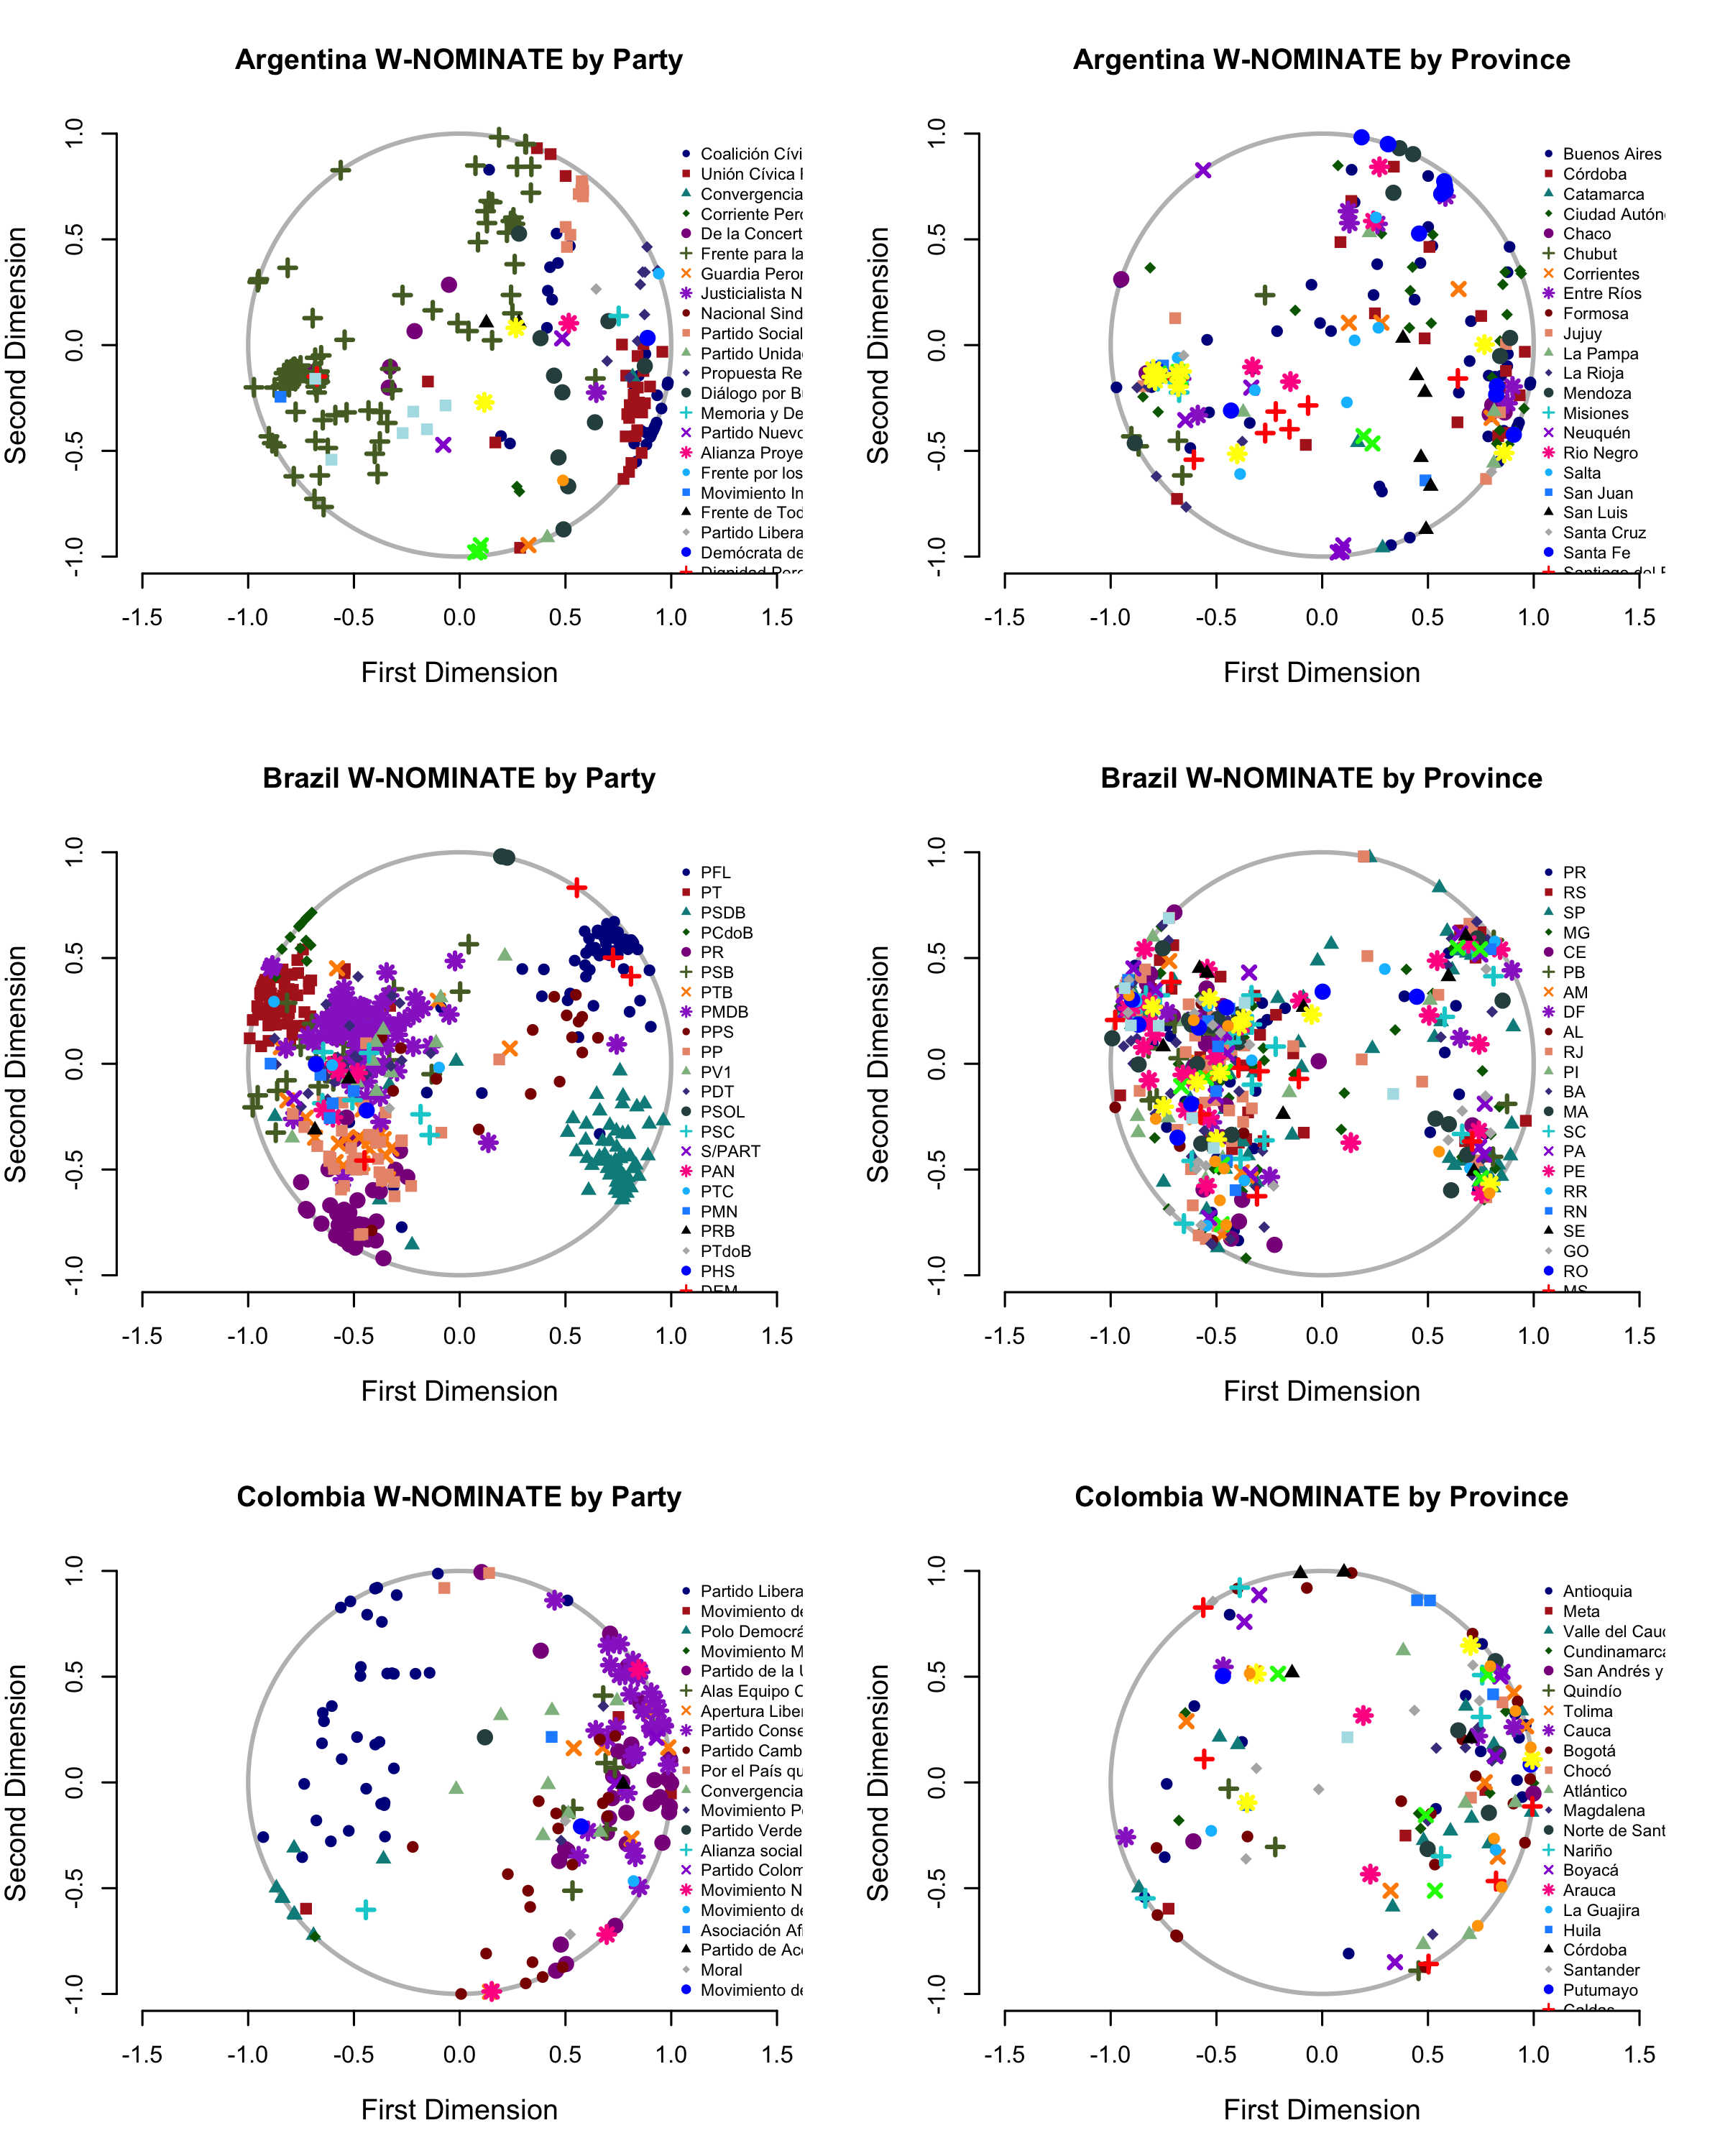
\includegraphics[width=17cm]{partyProvBehavior.png}
\label{fig:wnom}
\end{center}
\end{figure}

Looking at the Brazilian case, we can see that partisanship is a much stronger indicator of legislators' behavior than province of origin. The large clusters inform us that legislators belonging to the same parties had very similar voting patterns in roll calls throughout the term. In contrast, the figure on the left shows the exact same ideal point estimates, but colored according to province of origin. In that case, points of all shapes and colors seem to be almost randomly distributed across the chart, indicating that this classification system is not likely connected to how legislators decide on bills. For instance, to the left, we see that the state of PE (Pernambuco), indicated by six-pointed, pink stars, has legislators above and below zero in both dimensions. This informs us that politicians from Pernambuco state have very distinct voting patterns. The interpretation for the Argentinian and Colombian cases is similar, although partisan behavior seems slightly weaker. Also, in Argentina, there is an identifiable degree of provincial behavior related specifically to Santa Fe and Mendoza, on the far right of the circle. A general interpretation of these scores indicates that legislators do not necessarily vote according to conflicting interests between sub-national units, but following an ideological (partisan) standpoint.

Thus, if legislators do not vote provincially, we have reason to believe that malapportionment would have an effect on voting outcomes if provinces have very different party preferences. In this case, a province that is over-represented by the rules of malapportionment may be benefiting a specific party to gain more seats than it should. Along the same lines, the underrepresentation of a state may be reducing the seat share of a party that could otherwise be much stronger. Thus, parties may function as the mediator for the effects of province-based malapportionment. The reason for shifting decisions would not necessarily be that states have competing interests, but the fact that their majorities have opposing ideologies.

Although Figure \ref{fig:wnom} is informative on its own, we cannot directly infer that sub-national units have no influence on the \textit{ideo-lite} position of legislators. To confirm that this is the case, I run variance analyses\footnote{To see the full results, please refer to the \hyperlink{https://github.com/catarinaroman/malapportionment-lat-am/appendix.pdf}{Appendix}.} on the first and second dimensions of the W-NOMINATE scaling out the influence of party labels and province of origin. The results confirm the straightforward interpretation of the W-NOMINATE plots. Partisanship is a stronger predictor of legislative behavior than provincialism. This trend is observable in parliament dynamics where sub-national unit leaders are often not official entities, while parties and party-leaders hold considerable power. Although provincial behavior is less pronounced than partisanship, Argentina presents a significant sub-national unit influence in both dimensions. This is likely due to the strength of its regional parties and blocks, in contrast with Colombia's weak regional politics.

Based on results so far, if malapportioning seats influences legislative outcomes, the reason behind it is differential party preference across sub-national units, and not necessarily provincial behavior. Tables \ref{tab:arg_party}, \ref{tab:bra_party}, and \ref{tab:col_party} present the estimated counterfactual distribution of seats among parties.

\begin{landscape}
\begin{table}[!htb]
\small
\parbox{.3\linewidth}{
\centering
\caption{Diff. Party Share: Malapportioned vs. Well-Apportioned Congress \\ (\textbf{Argentina})}
\label{tab:arg_party}
\scalebox{0.8}{
\begin{tabular}{lrrr}
  \hline \hline
 & Uncorr & Corr & Diff \\ 
  \hline
  Frente para la Victoria & 63 & 76 & 13 \\ 
  Democrata Progresista & 2 & 3 & 1 \\ 
  Frente Justicia, Union y Libertad & 2 & 3 & 1 \\ 
  Movimiento Popular Neuquino & 1 & 2 & 1 \\ 
  Alianza Frente de Todos & 2 & 2 & 0 \\ 
  Frente Civico y Social & 1 & 1 & 0 \\ 
  Una Nueva Opcion & 1 & 1 & 0 \\ 
  Accion por la Republica & 1 & 0 & -1 \\ 
  Concert. P/Una Sociedad Justa & 1 & 0 & -1 \\ 
  Concertacion UNA & 1 & 0 & -1 \\ 
  De la Concertacion & 1 & 0 & -1 \\ 
  Democrata Cristiano & 1 & 0 & -1 \\ 
  Democrata de Mendoza & 1 & 0 & -1 \\ 
  Frente Cordoba Nueva & 1 & 0 & -1 \\ 
  Frente de Todos & 1 & 0 & -1 \\ 
  Mov de Integracion y Desarrollo & 1 & 0 & -1 \\ 
  Partido Liberal de Corrientes & 1 & 0 & -1 \\ 
  Santa Fe Federal & 1 & 0 & -1 \\ 
  Solidaridad e Igualdad & 1 & 0 & -1 \\ 
  Union de Centro Democratico & 1 & 0 & -1 \\ 
  Union Peronista & 1 & 0 & -1 \\ 
  Afirmacion Para Una Rep Igualitaria & 6 & 4 & -2 \\ 
  Alianza Proyecto Sur & 3 & 1 & -2 \\ 
  Union Civica Radical & 13 & 11 & -2 \\ 
  Dialogo por Buenos Aires & 4 & 1 & -3 \\ 
  Partido Socialista & 6 & 3 & -3 \\ 
  Propuesta Republicana & 10 & 6 & -4 \\ 
  Coalicion Civica & 33 & 13 & -20 \\ 
   \hline \hline
\end{tabular}
}}
%\end{table}
\hspace{.5cm}
\parbox{.3\linewidth}{
%\begin{table}[!htb]
\centering
\caption{Diff. Party Share: Malapportioned vs. Well-Apportioned Congress \\ (\textbf{Brazil})}
\label{tab:bra_party}
\scalebox{0.8}{
\begin{tabular}{lrrr}
  \hline \hline
 & Uncorr & Corr & Diff \\ 
  \hline
PSB & 27 & 36 & 9 \\ 
  PSDB & 66 & 74 & 8 \\ 
  PDT & 24 & 26 & 2 \\ 
  PSOL & 3 & 5 & 2 \\ 
  PV & 13 & 15 & 2 \\ 
  PL & 23 & 24 & 1 \\ 
  PTC & 3 & 4 & 1 \\ 
  PAN & 1 & 1 & 0 \\ 
  PMN & 3 & 3 & 0 \\ 
  PRONA & 2 & 2 & 0 \\ 
  PFL & 65 & 64 & -1 \\ 
  PHS & 2 & 1 & -1 \\ 
  PRB & 1 & 0 & -1 \\ 
  PSC & 9 & 8 & -1 \\ 
  PT do B & 1 & 0 & -1 \\ 
  PC do B & 13 & 11 & -2 \\ 
  PMDB & 89 & 87 & -2 \\ 
  PP & 41 & 38 & -3 \\ 
  PTB & 22 & 19 & -3 \\ 
  PT & 83 & 79 & -4 \\ 
  PPS & 22 & 15 & -7 \\ 
   \hline \hline
\end{tabular}
}}
\hspace{.5cm}
%\end{table}
\parbox{.3\linewidth}{
%\begin{table}[!htb]
\centering
\caption{Diff. Party Share: Malapportioned vs. Well-Apportioned Congress\\ (\textbf{Colombia})}
\label{tab:col_party}
\scalebox{0.8}{
\begin{tabular}{lrrr}
  \hline \hline
 & Uncorr & Corr & Diff \\ 
  \hline
Polo Democratico Alternativo & 7 & 12 & 5 \\ 
  Partido Cambio Radical & 20 & 24 & 4 \\ 
  Movimiento Alianza Social Indígena & 0 & 1 & 1 \\ 
  Partido Colombia Democratica & 2 & 3 & 1 \\ 
  Partido Conservador Colombiano & 29 & 30 & 1 \\ 
  Huila Nuevo y Liberalismo & 2 & 2 & 0 \\ 
  Moral & 1 & 1 & 0 \\ 
  Movimiento De Participación Popular & 1 & 1 & 0 \\ 
  Movimiento Nacional & 2 & 2 & 0 \\ 
  Movimiento Nacional Progresista & 1 & 1 & 0 \\ 
  Movimiento Popular Unido & 2 & 2 & 0 \\ 
  Partido De Accion Social & 1 & 1 & 0 \\ 
  Por el Pais que Soñamos & 2 & 2 & 0 \\ 
  Movimiento De Integración Regional & 4 & 3 & -1 \\ 
  Movimiento De Salvacion Nacional & 1 & 0 & -1 \\ 
  Movimiento MIRA & 1 & 0 & -1 \\ 
  Movimiento Alas Equipo Colombia & 8 & 6 & -2 \\ 
  Movimiento Apertura Liberal & 5 & 3 & -2 \\ 
  Partido Convergencia Ciudadana & 8 & 6 & -2 \\ 
  Partido Liberal Colombiano & 35 & 33 & -2 \\ 
  Partido Social De Unidad Nacional & 29 & 26 & -3 \\ 
   \hline \hline
\end{tabular}
}}
\end{table}
\end{landscape}

The results show that Argentina's party distribution becomes more unbalanced with proportional apportionment. When the system is more proportional, the largest party -- Frente para la Victoria -- becomes overwhelmingly majoritarian and most smaller parties lose either all, or significant amounts of seats. This is an expected result, as malapportionment was deliberately envisioned to produce more consociative democracy. Outcomes are more balanced in the Brazilian case. The left-leaning government party PT (Worker's Party) loses some seats, but so does the opposition's PPS (People's Socialist Party). While the PSB (Brazilian Socialists) -- which forms a coalition with PT -- wins nine seats, the right-leaning PSDB (Social Democrats) wins eight. In Colombia, we see the smallest aggregate change. Most small parties do not lose seats. Based on the new partisan distributions of congress seats, we expect malapportionment to have a strong effect on Argentinian legislative outcomes, moderate effects in Brazil, and close to no effects in Colombia.

Figure \ref{fig:monte} shows the results of the Monte Carlo simulations. For each country, I test the full sample of simple majority bills on the left. To the right, I use a sub-sample of the highly competitive bills, where the decision was within a 60-40 split, where the marginal legislator is more relevant. The \textit{correct predictions} translate the share of roll call votes that had the same result in real congress and in the simulation. High percentages mean that malapportioned and well-apportioned chamber decisions were very similar, and that malapportionment barely changed legislative outcomes. Low percentages mean that the well-apportioned chamber's decisions differ from those of the actual assembly, and that malapportionment more significantly changed the course of lawmaking. 

%Correct predictions translate the share of simulated roll call voting outcomes in the counterfactual congress that equal the original malapportioned chamber's decision. 

\begin{figure}[h]
\begin{center}
\caption{Simulation estimates}
\vspace{.3cm}
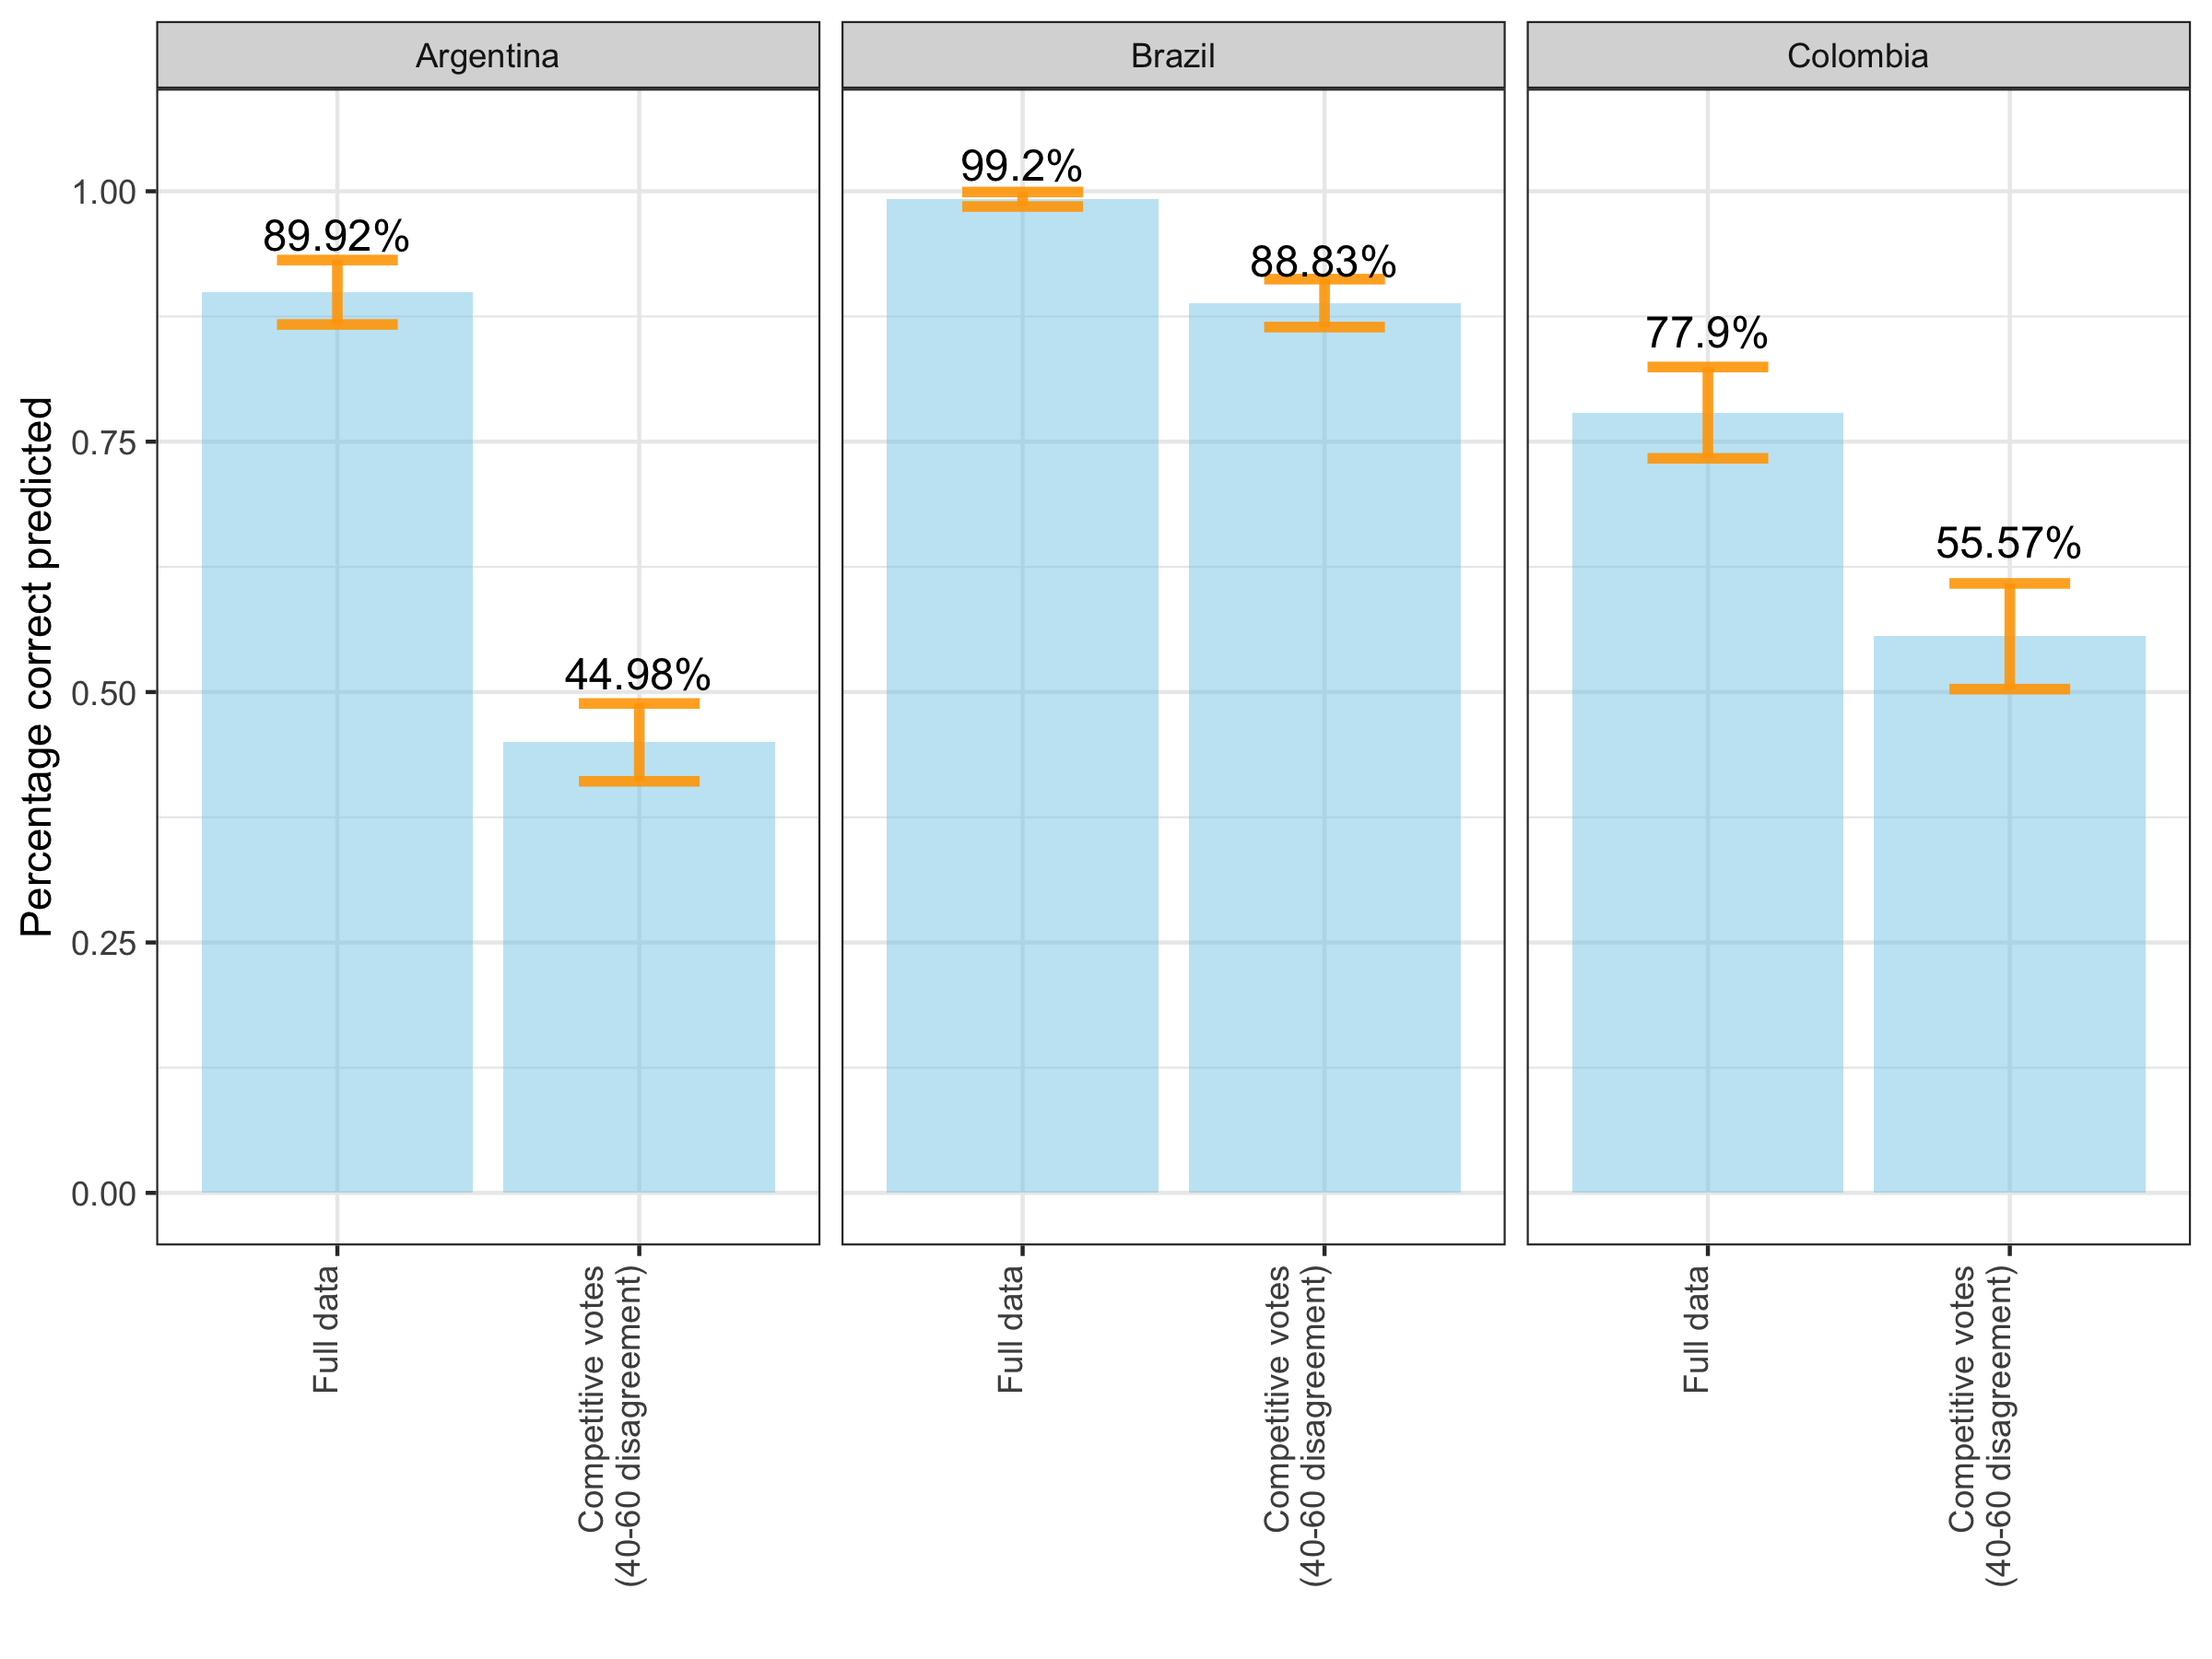
\includegraphics[width=17cm]{simvots.png}
\label{fig:monte}
\end{center}
\end{figure}

Argentina's \textit{Camara de Diputados} voted on 238 laws between 2008 and 2010, and approved all but six. Twenty-two (9.24\%) were competitive, and simple majority approved 21 of them. Our simulated floors resulted in the same voting outcomes as the real Argentinian congress in 89.92\% of the time. But when it comes to actually competitive legislation, only 44.98\% of bills would have the same outcome. Brazil's \textit{Câmara dos Deputados} voted 280 bills between 2007 and 2010, and approved 135, rejecting 146. The Brazilian case is thus more unpredictable because the Executive sends bills to the congress floor without properly weighing how they will be received \citep{ames2002deadlock}. The counterfactual congress would vote just like the malapportioned congress 99.2\% of the time. Looking only at competitive bills, the theoretical congress would agree with the decision in about 13 of the 15 voted by the real congress. Thus, correcting malapportionment in Brazil would likely not spark big changes in legislative activity.

Colombia is the most surprising case, as the direct interpretation of the Monte Carlo simulations goes against the expectations that malapportionment would have weak effects. The Colombian \textit{Congreso} voted 250 laws between 2007 and 2010, approved 107, and rejected 143. Of the 28 competitive bills, 8 were approved. The well-apportioned congress would disagree with the original congress' choices 22.1\% of the time in the full sample of simple majority bills. Yet, 44.43\% of competitive bills could have alternative outcomes in the counterfactual distribution of seats. This is unexpected since, compared to the other two countries, the distribution of seats between parties did not drastically change. The results, then, indicate that malapportionment has negligible effects for Brazil, but can significantly influence lawmaking in Argentina and Colombia. 

%%% Umberto, de onde vieram esses 71.4????

%Nevertheless, the model predicted 55.6 percent of the competitive bills, which is better than the Argentinian predictions, but still worse than the actual 71.4 percent of the random guess that all bills would fail to be approved. 

\section{Discussion}
\label{sec:discussion}

The Argentinian, Brazilian and Colombian cases show that malapportionment distorts representation under specific party system conditions, and when it is present past certain levels. %The most intuitive insight in this study is that more malapportionment generates more results that differ from a better-apportioned counterfactual. 
We see this as Argentina and Colombia, whose indexes were .14, had stronger malapportionment effects than Brazil, whose index was only .05. Yet, there are a few particularities to each country that must be addressed. In simple-majority roll call voting, especially in the analysis of competitive bills, the marginal legislator has decisive power. Hence my effort in designing an accurate rule to predict individually how the new legislators who compose congress would vote. This is a key point in the methodology, as the utility I attribute to these theoretical legislators derives directly from the party and province scores I measured in the W-NOMINATES. Yet, if party behavior is not homogeneous, the party scores may not accurately translate the position of partisans. This means there is a degree of particularism that estimates cannot capture, which makes predictions less precise. While the three scenarios are comparable for being PR systems, their open and closed-list electoral rules, and unique party dynamics must be taken into account to interpret the simulation results. 
%Thus, there are specific features of these countries' party and electoral systems we must take into account to interpret the simulation results.

Argentina presented the strongest, most straightforward results to support my hypothesis. Correcting the distortions in the chamber of deputies changes the distribution of seats among parties. This cancels out consociational democracy efforts by making small parties disappear. It also reflects a scenario where the opposition is not effective, constituting a tyranny of the majority based on \textit{Frente para la Victoria}'s winning coalition. Even so, the provincial effect is not negligible. Argentina has strong sub-national party systems operating alongside and within the national party system \citep{gibson2010federalized}. %This means that, not only are sub-national political systems autonomous, but they are also highly influential over national politics. 
This helps us understand why, for Argentina, provinces have a stronger input on decisions according to the W-NOMINATE ANOVA analysis.\footnote{Please refer to the full results of variance analysis on the Appendix.} %The strength of sub-national party systems also explains why the absence of small parties from the counterfactual congress produces such different decisions from the real congress.
Roll call vote outcomes thus change considerably due to the strength of sub-national party system and of the winning coalition.

%The Brazilian and Colombian cases are the most enlightening once we compare one with the other.

Comparing Brazil to Colombia sheds light on counterintuitive dynamics that take place in each country, making them all the more interesting. %Brazil and Colombia become especially interesting when compared. 
While Brazil is an open-list PR system, Colombia elects representatives through closed-lists. Highly personalistic campaigns and candidates generally manifest in open-list PR, translating heated intra-party competition \citep{mershon2020challenging}. Party leaders have great difficulty in disciplining elected politicians whose platform and strategy are truly personalistic. Thus, in open-list PR, we should observe heterogeneous party behavior in congress roll call votes. In closed-list PR, intra-party competition would be much less rampant during elections, and voters would not witness it in campaigns. Instead, it would have taken place \textit{before} the election, when the party forms its list(s).

Brazil and Colombia inverse the open versus closed list pattern, and the results presented here corroborate this idea. I find regionality is not significant in either country. In Brazil, most party leaders can discipline their politicians almost perfectly, and intra-party competition is moderate \citep{figueiredo2000presidential}. \cite{desposato2006impact} is among the studies that demonstrate that the Brazilian lower chamber does not entirely suffer from the malicious open-list PR effects reported in the classic electoral system literature. Recent findings show that the number of effective running candidates is low, and that they are mostly members of large parties who coordinate to maximize the number of seats awarded to the label as a whole \citep{cheibub2020preference}. In spite of malapportionment, partisan seat distribution remains balanced compared to the counterfactual correction, and parties effectively discipline their incumbents. Thus, a reform to reduce distortion would not be highly beneficial -- as the real outcomes are not far from those of an ``ideal'' apportionment.

\citet{leongomez2006giants} finds the Colombian party system in 2006 is fragmented with personalistic and undisciplined legislators. This explains the number of "independent" parties, whose officeholders often abstain from openly aligning with either the government (conservatives) or the opposition (liberals). Legislators' disloyalty to parties may also be an individual signaling strategy to extremist constituents, as \citet{kirkland2018roll} suggest happens in British and American assemblies. Each party can launch as many lists as it likes, and most lists elect only the first candidate.\footnote{For instance, in 2002, of the 321 lists running for the upper house, only 3 elected more than one senator \citep{leongomez2006giants}.} Citizens thus vote for the list head, who is not coordinated with other candidates from their label. 

W-NOMINATE estimates reflect the indiscipline of Colombian legislators visually: we do not see clusters of party behavior as markedly as for the other two countries. This is because politicians in the same party act autonomously, which translates into heterogeneous voting patterns. Moreover, if partisanship is but a pretext \citep{leongomez2006giants}, the party scores may not generate very accurate predictions of behavior, which affects the simulation results. If the scores I based on are not highly predictive, the constructed legislators for the well-apportioned chamber may be too disordered. Besides, one can also argue that the Colombian results are the least conclusive, since Colombia's index after correction is actually very close to Brazil's starting malapportionment index.

Moreover, the cleavages dividing Colombian politics have their axis around the first dimension (right- left- positions) in Figure \ref{fig:wnom}. We can clearly see former President Uribe's coalition, composed of the Conservative Party, the ``U'' Party (\textit{Partido Social de Unidad Nacional}), the Radical Change Party (\textit{Cambio Radical}), and the Liberal Opening Movement (\textit{Apertura Liberal}), occupying the right half of the plot. On the left, are the Liberal Party and the Alternative Democratic Pole (\textit{Polo Democrático Alternativo}, the FARC party). The winning coalition seems incontestable in Colombia when it comes to central matters such as national security and the state's strategy to combat militias. Thus, it must be acknowledged that the highly competitive bills from Colombia may be low-yield issues, or centered around the second dimension axis, such as minority rights. Although malapportionment may alter these voting outcomes, the bills that shape national politics may not be affected by the disproportionate seat distribution. 


\section{Conclusion}
\label{sec:conclusion}

In this paper I evaluate whether malapportionment in national congresses changes legislative outcomes. I analyze the cases of three PR systems (Argentina, Brazil, and Colombia) during the period of 2007-2010. I find that some characteristics of each political system have considerable influence on the scale of malapportionment effects. Party politics play an especially important part, since majority formation determines decision-making in assemblies. It is important to note that the results here represent a partial-equilibrium analysis. It dismisses the conjecture that, under different electoral rules, parties', politicians', and voters' strategies would be different, and perhaps so would their agendas. Yet, the exercise I perform remains valid, as I measure the impacts of malapportionment against a reapportioned counterfactual that purely corrects distortions. It is shown to be an adequate method to assess the impact that malapportionment can have on lawmaking.

This paper makes three contributions to the scholarship. First, it empirically identifies how some electoral rules affect representation \citep{carey2011electoral, pierzgalski2018balancing} and other institutional features, such as accountability \citep{myerson1993incentives}, public good provision \citep{lizzeri2001provision}, and even corruption \citep{persson2003electoral}. Second, the paper advances the literature on malapportionment and its effects, following \citet{mignozzetti2011faz} in the Brazilian case. Third and last, I add to a broader research effort employing partial-equilibrium simulations to evaluate the effects of institutional features, demonstrating how they can be used in the case of legislator distribution. 

This study, however, does not perform a predictive evaluation of reapportionment reforms. Because it does not address all of the costs reform incurs, I advise against its direct use to motivate, or to discourage institutional change. As I have pointed out, real world political negotiation would most certainly veto naïve corrections. End results would likely be an immense increase in the size of national chambers, in which case, my results do not necessarily apply. Although a recent meta-analysis \citep{alptekin2020effect} shows that larger chambers do not necessarily spend more, they might produce other forms of resource misallocation, especially in countries plagued by corruption and high coordination costs. Building on this point, I highlight the importance of a qualitative assessment of the bills to evaluate the scope and scale of the transformations that reapportionment could produce. This paper may be used as a stepping stone for further investigation, so that future endeavors might estimate what real proposals to reapportion legislative chambers could and should look like.


\newpage
\bibliography{references.bib}
\bibliographystyle{apalike}

\newpage

\section{Online Appendix}

\begin{table}[!htb]
\centering
\caption{Brazilian Party Labels}
\label{tab:party_labels}
\scalebox{0.8}{
\begin{tabular}{rl}
  \hline \hline
Acronym & Name \\ 
  \hline
PSB & Brazilian Socialist Party \\ 
  PSDB & Brazilian Social Democratic Party \\ 
  PDT & Democratic Labor Party \\ 
  PSOL & Socialism and Liberty Party \\ 
  PV & Green Party \\ 
  PL & Liberal Party \\ 
  PTC & Christian Labor Party \\ 
  PAN & Party of the Nation's Retirees \\ 
  PMN & Party of National Mobilization \\ 
  PRONA & Party of the Reconstruction of the National Order \\ 
  PFL & Democrats (Liberal Front Party) \\ 
  PHS & Humanist Party of Solidarity \\ 
  PRB & Republicans (Brazilian Republican Party) \\ 
  PSC & Social Christian Party \\ 
  PT do B & Worker's Party of Brazil \\ 
  PC do B & Brazilian Communist Party \\ 
  PMDB & Brazilian Democratic Movement Party \\ 
  PP & Progressives (Progressive Party) \\ 
  PTB & Brazilian Worker's Party \\ 
  PT & Worker's Party \\ 
  PPS & People's Socialist Party \\ 
   \hline \hline
\end{tabular}
}
\hspace{.5cm}
\end{table}

\begin{table}[!htb]
\centering
\caption{Brazilian State Acronyms}
\label{tab:brastates}
\scalebox{0.8}{
\begin{tabular}{rl}
  \hline \hline
Acronym & State name  \\ 
  \hline
AC & Acre \\ 
  AM & Amazonas \\ 
  AP & Amapá \\ 
  DF & Distrito Federal \\ 
  MS & Mato Grosso do Sul \\ 
  MT & Mato Grosso \\ 
  RN & Rio Grande do Norte \\ 
  RO & Rondonia \\ 
  RR & Roraima \\ 
  SE & Sergipe \\ 
  TO & Tocantins \\ 
  AL & Alagoas \\ 
  ES & Espírito Santo \\ 
  PI & Piauí \\ 
  PB & Paraíba \\ 
  SC & Santa Catarina \\ 
  GO & Goiás \\ 
  PA & Pará \\ 
  MA & Maranhão \\ 
  CE & Ceará \\ 
  PE & Pernambuco \\ 
  PR & Paraná \\ 
  RS & Rio Grande do Sul \\ 
  BA & Bahia \\ 
  RJ & Rio de Janeiro \\ 
  MG & Minas Gerais \\ 
  SP & Sao Paulo \\
   \hline \hline
\end{tabular}
}
\end{table}

\end{document}
